\chapter{State-of-the-Art Interconnects}
\label{ch:state}
Nowadays the Peripheral Component Interconnect Express (PCI Express) and AXI are the interconnect industry standard for PC and server systems, and embedded platforms, respectively. Recently, three open initiatives were announced: CCIX, Gen-Z and OpenCAPI. These open standards are all driven by ISA-agnostic tighter coupling of processors and accelerators, by enabling direct memory access between compute resources and reducing data movement. Also new and emerging memory and storage technologies are exploited \cite{benton}.\\
This chapter focuses on interconnects targeted for accelerators, network, and memory and storage solutions. However, specific memory and storage features of such interconnects will not be discussed. Also interconnects tailored for specific domains such as Ethernet and InfiniBand for networking, NVLink for GPUs and Gen-Z for storage are not discussed, nor are SMP protocols.

%\todo{
%- research transactional memory, would it solve some problems? allows for load/store ops to execute atomically. interesting for parallel systems.\\
%- decide on model of the system, see comparison paper and CAPI UG (asynchronous pull model by afu). OpenCAPI diverted from these models in the architecture because not everyone was using them. So now the philosophy is to let the AFU designer choose the WED model of operation. More info in email conversations with Curt.\\
%- Section on the WED model and other parallel models. Also compare to other accelerator programming models such as CUDA.\\
%- Interesting aspect is how FPGA acceleration looks like for a programmer. What is the typical programming model / paradigm? Or is this captured in 'Need for Shared Memory and Coherence' section? CAPI uses WED, PCIe uses DMA I think, OCAPI uses nothing in particular.
%}





\section{PCI Express}
PCI Express has been around since 2003 and gone through several generations. The PCI-SIG is a group of over 900 companies that maintain the standard. Currently the most widely adopted generation is number three and generation four compliant devices are slowly being released. The remainder of this section briefly explains the architecture of PCI Express and summarises key features of current and future generations.

%\todo{
%- pcie endpoint: is the cpu always the master of the pcie bus, or can a gpu for example also take over? or is it not master-slave style? i remember they always talk about endpoints of pcie root complex.\\
% Endpoint can be the bus master, some information can be found here: \url{https://forums.xilinx.com/t5/Welcome-Join/how-does-a-PCIE-endpoint-recived-master-privilege/td-p/779945}.\\
%- PCIe protocol overview: \url{http://www.ni.com/white-paper/3767/en/}: "The run-time software model used by PCI is a load-store, shared-memory model, which is maintained within the PCI Express architecture to enable all existing software to execute unchanged.".\\
%}



\subsection{Architecture}
This section explains the architecture of PCI Express Gen 3 and later, since various changes have been made at the packet level compared to previous generations of PCI Express which will not be discussed.\\
PCI Express is a packet-based, split transaction protocol with a point-to-point or switched topology. Split transaction means that a request and response are separated by time. Each device is connected to the root complex. The root complex is the root of the IO hierarchy and is connected to the processor and host memory. A PCI Express bus link supports full-duplex communication between two endpoints, with no inherent limitation on concurrent access across multiple endpoints. It uses credit based flow control and typically each link consists of one, four, eight or sixteen lanes. Legacy PCI features are backwards compatible with PCI Express.



\subsubsection{Protocol Description}
The PCI Express architecture consists of three logical layers called the Transaction Layer, the Data Link Layer, and the Physical Layer \cite{pcie-intel}. \autoref{fig:3-pcie} shows a layering diagram and the receive (RX) and transmit (TX) channels of the architecture. Each layer will be briefly discussed.\\
PCI Express uses packets to communicate between participants of the link. Packets are formed in the Transaction Layer and are extended with additional fields when passing through other layers. These additional fields contain information required by other layers to handle the packet appropriately. The receiver of a packet removes these fields in reverse order and uses the information.

\begin{figure}[H]
  \centering
  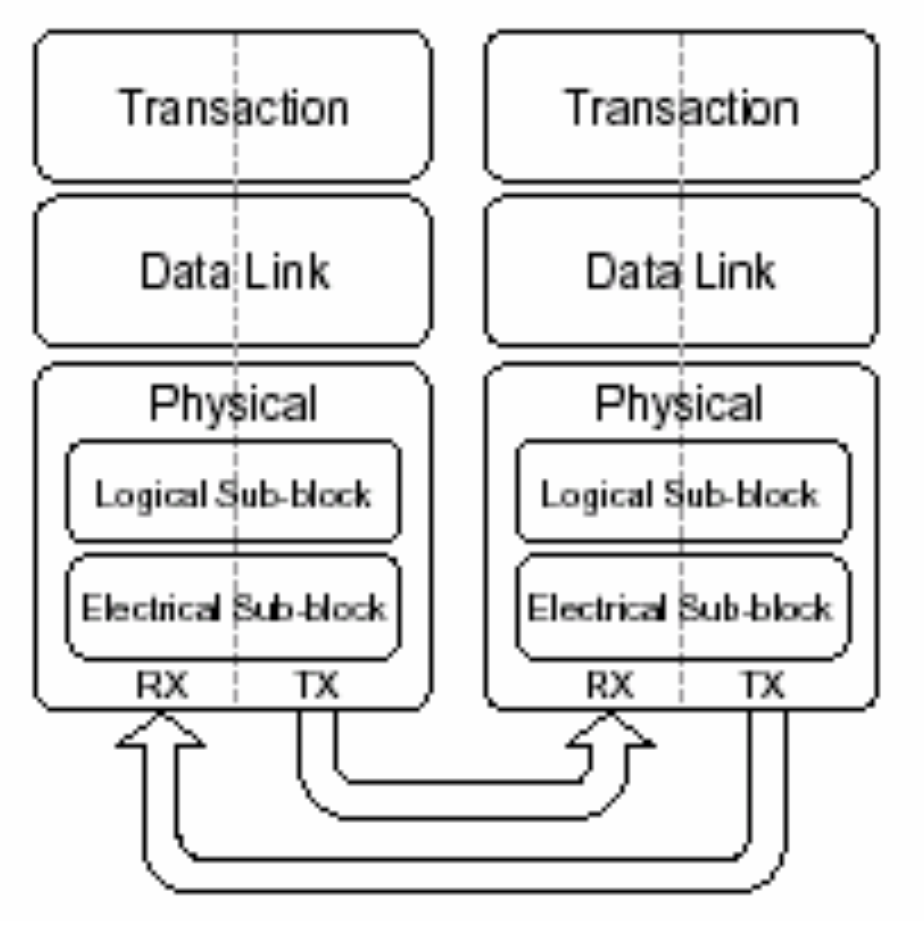
\includegraphics[width=0.40\textwidth]{3-pcie.png}
  \caption{Layering diagram of the PCI Express standard \cite{pcie-intel}.}
  \label{fig:3-pcie}
\end{figure}

\autoref{fig:3-pcie} shows the layering diagram of the PCI Express standard. The Transaction Layer is the top layer and assembles and disassembles Transaction Layer Packets (TLPs). TLPs are the packets used to communicate information and data between two endpoints and consist of a header and data part. Also flow control is managed by using a credit-based scheme and ensures that TLPs are only transmitted when a buffer is available on the other endpoint. This eliminates wasting bandwidth on packet retries due to resource constraints.\\
The Data Link Layer is the middle layer and tags TLPs and handles error detection and correction. The transmission side of this layer pre-pends a sequence number (tag) to the TLP and appends a CRC field to it. The receiving side validates the sequence number, by checking if it is continuous with the sequence number from the previous TLP. It also validates the data by checking the CRC. If the TLP is valid, an acknowledgement (ACK message) is sent to the transmitter. If one or both are invalid, a NAK message is sent and re-transmission of all TLPs starting from the invalid one is requested. The ACK and NAK messages are communicated between layers as Data Link Layer Packets (DLLPs).\\
The Physical Layer is the lowest layer and consists of both electrical circuitry, such as a serialiser/deserialiser (SerDes), and logical components to initialize the interfaces. A lane between two endpoints consists of two unidirectional differential signalling pairs and multiple lanes can be bundled together to form a link.



\subsubsection{Cache Coherency Snooping}
Originally proposed as an extension to PCI Express Gen 2, TLP Processing Hints (TPH) \cite{pcie-tph} provide hints for the host to improve memory access performance by taking the cache hierarchy into consideration. This is done by providing several bits in the TLP. The host snoops memory access requests from PCI Express attached devices to enforce cache coherency by hardware \cite{pcie3}.\\
However, these snoop hints are not required for every memory access request. An example is when a speculative read-ahead buffer is used by the operating system to access storage. Snooping this data could pollute host caches and, therefore, the TPHs can be configured on a per packet basis \cite{pcie3-intel}.

%\todo{
%- "standford ee282 lecture 9" page 24 shows what cache snoop does.\\
%- PCIe Gen 3 spec: page 76 talks about cache coherence (snoop).\\
%- PCIe supports memory request snooping in order to keep CPU caches coherent. \url{https://www.embedded.com/design/connectivity/4008241/1/PCI-Express-Gen-3-Simplified}\\
%- Caching hints explanation: \url{https://www.intel.sg/content/dam/doc/white-paper/pci-express3-accelerator-white-paper.pdf}\\
%}



\subsubsection{Address Translation Services}
Another extension proposed for PCI Express Gen 2 are the Address Translation Services (ATS) \cite{pcie-ats}. This extension was included in the PCI Express Gen 3 specification and translates untranslated addresses to physical addresses. ATS enables attached devices to request address translation from the host in advance to alleviate potential congestion during times with intensive communication across the interconnect \cite{pcie3-intel}.\\
To relieve the host translation agent, the extension proposes attached devices to implement an address translation cache (ATC) on the device itself. This allows device designers to size the ATC depending on the usage model of the device. 

%\todo{
%- There are four address spaces: config, memory, io and message. Address Type (AT) Field Encodings (Untranslated, Translation Request, Translated, Reserved) are explained in Address Translation Services Specification.\\
%}



\subsubsection{Atomic Operations}
Atomic Operations \cite{pcie-atomic} also have been added as an extension to PCI Express Gen 2 and were incorporated in the PCI Express Gen 3 specification. Atomic operations are used as a locking mechanism for shared memory and as a means of communication between host and attached device to reduce overhead compared to traditional solutions \cite{pcie3-intel}. Three different atomic operations are supported: FetchAdd, Swap, and Compare-And-Swap.

%\todo{
%- Post question on StackOverflow on PCIe features such as coherency, shared memory, and what ATS for example adds as functionality.\\
%- PCIe extensions for: a locking mechanism for shared memory, hints to help a coherent processor more effectively handle I/O and memory and protocol efficiencies for mapping virtual to physical memory. However, the resulting improvements fall significantly short of creating a cache coherent version of PCI Express. \url{https://www.eetimes.com/document.asp?doc_id=1163775}\\
%What exactly defines a cache coherent protocol and what misses from this list?\\
%}



\subsection{PCI Express Gen 3}
\label{sec:pciegen3}
The third generation of PCI Express was introduced in 2010 \cite{pcie3} and introduced various changes at packet level compared to the previous generation. The theoretical bandwidth of a single lane is \SI{1.0}{\giga\byte\per\second} but in practice is lower due to encoding, packet and traffic overhead \cite{pcie-xilinx}. Latency characteristics are difficult to come by. A study conducted in the field of real-time Ethernet found highly variable results \cite{pcie-killer}. A network interface card is attached to an Intel i5 3550 processor, either in the graphics or IO PCI Express Gen 3 slot. The graphics slot is connected directly to the root complex of the processor while the IO slot is connected through the chipset. The impact of the location of the slot is clearly visible in the obtained latencies of \SI{1.38}{\micro\second} for the graphics slot and \SI{3.11}{\micro\second} for the IO slot. These results have been obtained by reading the clock register located in the network card. The latency is defined as the time passed between two consecutive read requests of the clock register.

%\todo{
%- In depth latency measurement: \url{http://literature.cdn.keysight.com/litweb/pdf/5989-4076EN.pdf}\\
%}



\subsection{PCI Express Gen 4}
In October 2017, the final specification for PCI Express Gen 4 was released, limited to members of the PCI-SIG \cite{pcie4}. The most significant improvement is the doubling of bandwidth to \SI{2.0}{\giga\byte\per\second} per lane while retaining compatibility with previous PCI Express generations.



\subsection{PCI Express Gen 5}
In June 2017, PCI Express Gen 5 was announced \cite{pcie5}. Not much information has been shared publicly besides the doubling of bandwidth to \SI{4.0}{\giga\byte\per\second} per lane compared to the previous generation. The information presented in \autoref{tab:comparison} on Page \pageref{tab:comparison} assumes that PCI Express Gen 5 supports all the features from previous generations.





\section{CAPI}
To address emerging workloads and inefficiencies present in the traditional IO model (see Chapter 2), IBM's POWER8 processor introduced the Coherent Accelerator Processor Interface (CAPI) in 2014. CAPI enables accelerators to be plugged into PCI Express slots and act as a coherent peer of other caches within the system memory hierarchy \cite{capi_ibm}. CAPI also allows data to be referenced by an effective address in the same way as an application running on the host processor without the need for a device driver. A generic kernel extension enables CAPI in the host operating system. This removes software overhead, traditionally present for a software thread running on the host processor to share data with an attached device.
%Typically the only way to attach accelerators coherently was by using 'in-socket' accelerators, by using the HyperTransport for AMD or FSB/QPI/UPI for Intel. The main problems with this approach are that sockets are proprietary form factors and that a CPU socket is sacrificed. The need for coherency was shown before and IBM's CAPI for POWER8 enables coherent attached accelerators by leveraging the widely adopted PCIe standard and adding additional layers on top of it. By sharing the same address space as the CPUs, attached devices appear as a peer to the processor cores.\\
%In a nutshell, the CPU sets up the required data and calls the accelerator. The FPGA can then read and write coherent data across the PCIe interconnect. Additional logic is required on both ends of the PCIe interconnect. On the processor side, there is the CAPP logic which is the bridge between the POWER8 cores and the PCIe link. On the FPGA, the PSL is present which provides an interface and coherent cache to the accelerator.\\



\subsection{Architecture}
PCI Express does not natively allow attached devices to operate as a coherent peer, since it has no notion of the coherency protocol used within the host processor. To bridge both protocols, a hardware proxy unit, called the Coherent Accelerator Processor Proxy (CAPP), resides within the host processor and is connected to the coherent fabric as shown in \autoref{fig:3-capi}. Besides the CAPP, also the PHB is present within the host processor and provides the necessary hardware for the underlying PCI Express protocol used.
%The Coherent Accelerator Processor Proxy (CAPP) unit, in conjunction with the PHB, act as memory coherence, data transfer, interrupt, and address translation agents on the SMP interconnect [9] fabric for PCIe-attached accelerators.
The attached device, either an ASIC or FPGA, contains the POWER Service Layer (PSL) and one or multiple Accelerator Function Units (AFUs).

\begin{figure}[H]
  \centering
  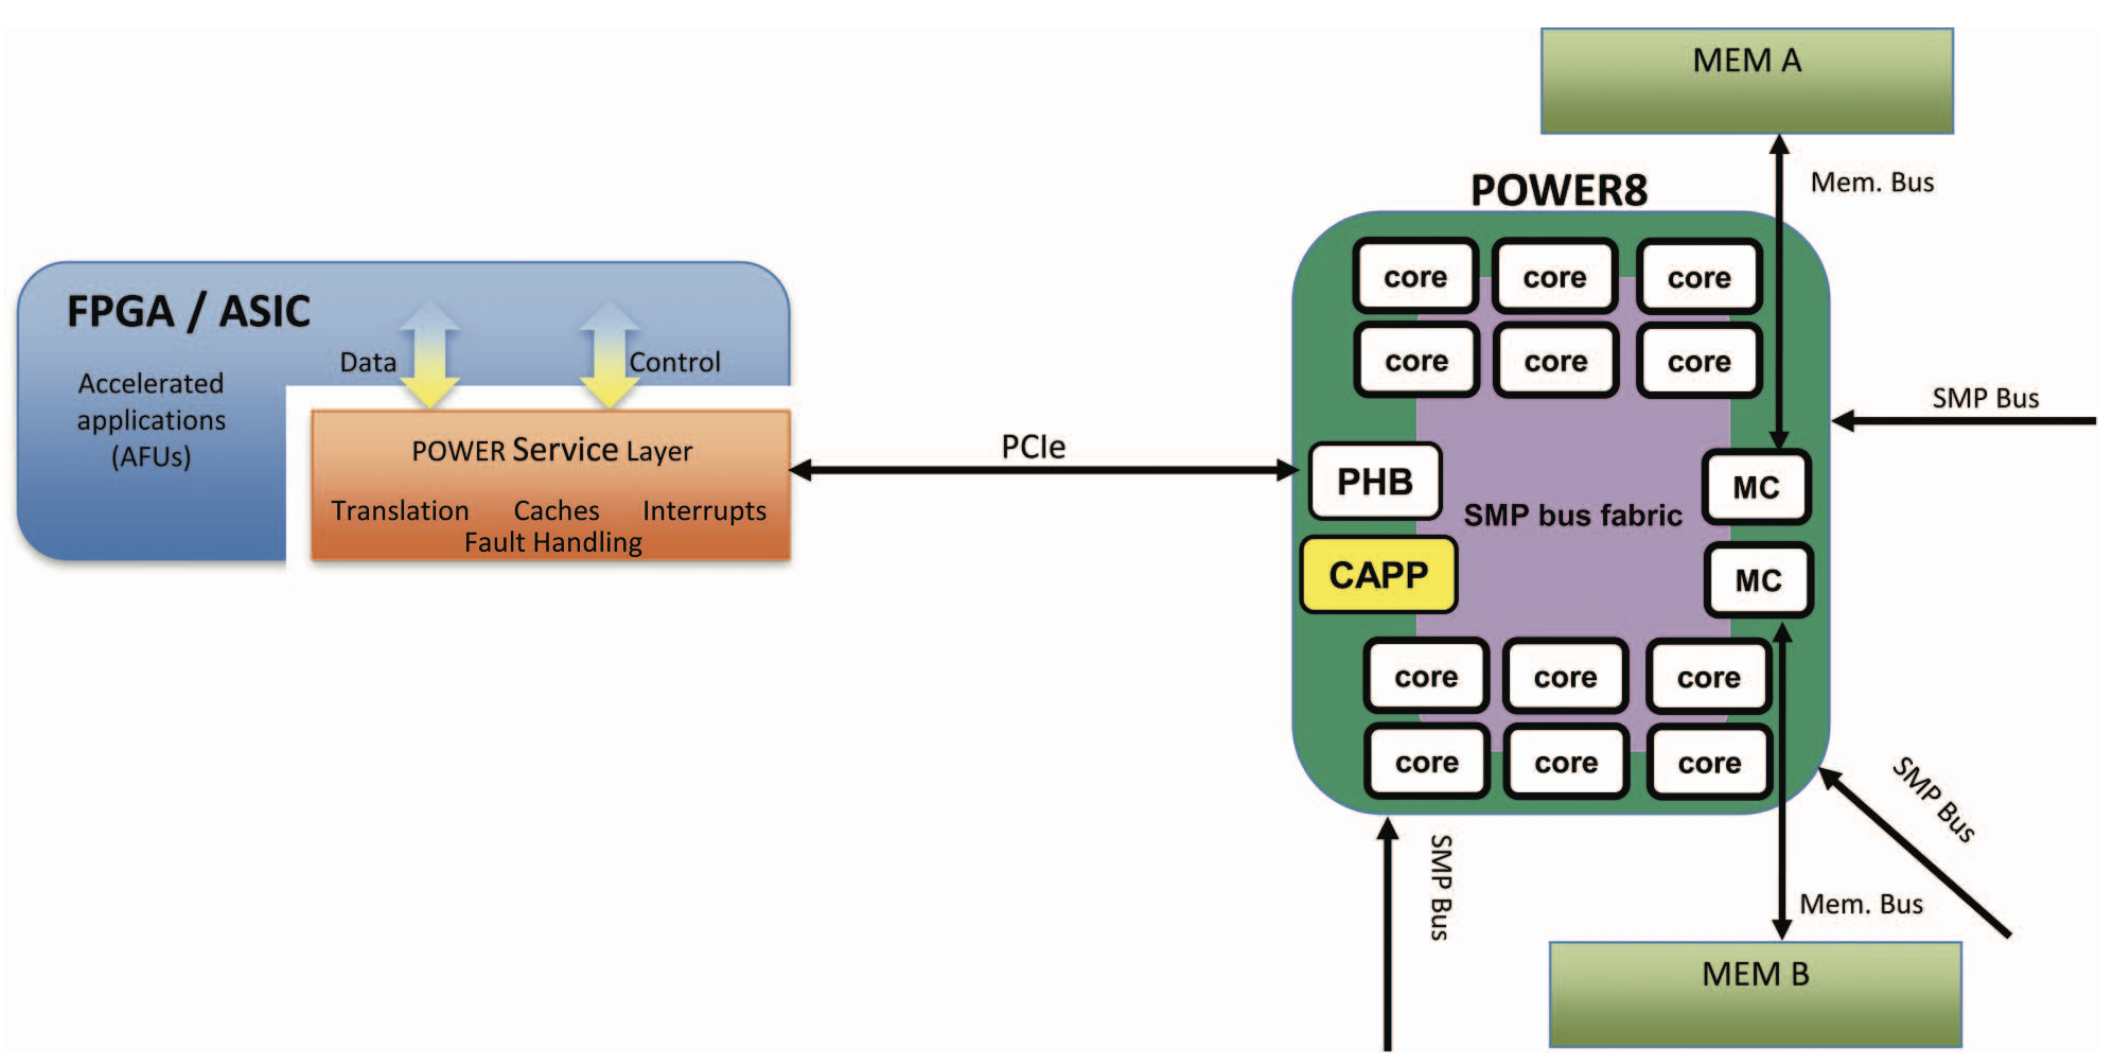
\includegraphics[width=0.85\textwidth]{3-capi.png}
  \caption{System architecture of a CAPI attached device \cite{capi_ibm}.}
  \label{fig:3-capi}
\end{figure}

When the CAPP, PHB, PCI Express and PSL are combined, the AFU is able to operate coherently on data in host memory. To reference the requested memory, the AFU uses effective addresses that are translated by a memory management unit (MMU) within the PSL. The PSL may also send interrupts to the host processor on AFU completion or to indicate a translation fault.\\
The interface provided by the PSL to the AFU hides cache coherence complexities and address translation. AFUs request host memory using a load-store model to user space effective addresses. Requests can be either cacheable or write-through (not cached). Cacheable requests are typically used to communicate control information between multiple processes and can be stored within a \SI{256}{\kilo\byte} cache within the PSL \cite{capi-white}. Write-through requests are typically used for data manipulation outside of the coherence domain and therefore require less messages to be transmitted over the PCI Express link and reduce overhead.\\
The programming model requires the application to setup data for the attached device in host memory, and to notify the AFU when the data is ready to be consumed. It is not possible to transfer data from the host processor to the AFU directly because the AFU has to master read and write commands for data located in host memory \cite{capi-bw}. The AFU can be notified in two different ways, either the AFU polls a location in host memory or the application running on the host writes into a specific MMIO register on the attached device.



\subsubsection{Coherence}
Coherent host memory access is enabled by a combination of the CAPP and PSL and both contain cache lines used by the AFU. The CAPP acts as a proxy for the PSL and snoops coherence messages on the fabric. Snoops that hit cache lines present in the CAPP could generate messages, transmitted across the PCI Express link, for the PSL. Coherence enables an AFU to cache data from host memory and to request locks to implement atomic operations for example \cite{capi-manual}.



\subsubsection{Address Translation}
In order for the AFU to operate on effective addresses, the PSL consists of an MMU that uses the host processor's page tables \cite{capi-zurich}. This enables AFUs to de-reference pointers, similar to a thread running on the host processor. System software manages page faults \cite{capi-white}. The MMU performs address translations and caches recent translations, in order to avoid page table walks. The CAPP also snoops translation invalidation messages from the fabric since the PSL consists of a translation cache.

%\todo{
%- Yvo: Subho, you mentioned that you had used CAPI and found that the locks present in the protocol where rather slow, or something along those lines. For my master thesis, I am looking into OpenCAPI, which uses atomics instead. I was wondering if you could provide me with more information about why the locks in CAPI where not as fast as desired and how you worked with this.
%Subho: I dont think the performance is a problem. The problem is that if you use the C++11 or POSIX locks in the software side, it is not quite clear how the locking protocol is implemented. So when we try to implement the the CAPI side of things, it becomes difficult to first understand the LINUX implementation and then figure out how to do something similar in hardware.
%In any case, high contention locks are a really bad. As FPGA very rarely gets the lock since it is much slower. I would advise using test and test and set based protocols along with priority to reverse the effects from the slow clock speeds in the FPGA.
%- Lance Thompson slides OpenCL CAPI: CAPI is shared virtual memory. Shared buffers can directly be instantiated instead of issuing memcpy functions.\\
%- great slides on PCIe versus CAPI from: Enabling Coherent FPGA Acceleration - Allan Cantle\\
%- has cache coherency\\
%- basically, WED concept exists in CAPI 1 (see CAPI UG), but no specifics regarding how this struct looks are defined.\\
%}

%\todo{CAPI interface summary from \url{https://www.xilinx.com/support/documentation/application_notes/xapp1293-amba-axi4-to-ibm-capi-adapter.pdf}\\
%The power service layer (PSL), is used by the accelerator to interface with the POWER8 system. It offers cache-line oriented services to an accelerator by way of five independent interfaces:
%- Control interface: The interface that allows the main application on the host to start, stop or reset the accelerator.
%- Command interface: The interface that is used by the accelerator to send read/write host memory requests.
%- Response interface: The interface that is used to acknowledge the accelerator about the completed commands.
%- Write buffer and read buffer interface: The interface that is used by the accelerator to send and receive data to, or from, the host memory.
%- MMIO interface: The interface that is used by the main application on the host to access the registers within the accelerator.

%There is a READY/VALID handshake in the PSL for flow control support. The data/responses are not always returned to the accelerator in the same order as the commands are issued.
%}

%\todo{From \url{http://events.linuxfoundation.org/sites/events/files/slides/lcjp15_mackerras.pdf}\\
%Two types of AFU for CAPI:
%“Dedicated” AFU can only be used by a single application
%“Directed” AFU supports multiple contexts and can be used by several applications concurrently
%}



\subsection{CAPI 1.0}
\label{sec:capi-1.0}
The first generation of CAPI was introduced with the IBM POWER8 processor in 2014 \cite{capi-white}. Since there is only one CAPP unit per POWER8 processor, the number of attached CAPI 1.0 devices is limited by the number of processors in the system. To improve adoption, Xilinx released an AXI4 to CAPI 1.0 adapter \cite{xilinx-xapp1293}.\\
The total bandwidth available to a CAPI 1.0 attached device is determined by the underlying PCI Express Gen 3 interconnect and the number of lanes. CAPI 1.0 supports eight or sixteen lanes per attached device \cite{opencapi-enablement}. The online CAPI Developers Community used a Nallatech P385-A7 FPGA attached using an eight lane PCI Express Gen 3 interface in conjunction with a POWER8 S824 system to assess the bandwidth and latency of CAPI 1.0 \cite{capi-bw}. The measurements were obtained using a modified \textit{memcpy} demo supplied with the developer kit. When data resides in host memory, a read bandwidth of \SI{3.42}{\giga\byte\per\second} was achieved with an average latency from PSL request to response of \SI{864}{\nano\second}. Similarly, write bandwidth of \SI{3.88}{\giga\byte\per\second} with an average latency of \SI{838}{\nano\second} was achieved. Reads and writes that hit in the PSL cache achieved a latency of \SI{120}{\nano\second}.\\
Due to the protocol overhead of CAPI 1.0 on top of PCI Express Gen 3, the obtained bandwidth is significantly less compared to the theoretical capabilities of PCI Express Gen 3. On the flipside, CAPI 1.0 provides several features and usage models that are not possible with a traditional PCI Express Gen 3 interconnect.

%The datasheet of the FPGA \cite{nalla-fpga} used states that the device is tested at PCI Express Gen 3 speeds, but by default operates at Gen 2 speeds. The simplex bandwidth for Gen 2 is \SI{4.0}{\giga\byte\per\second}. This explains the relatively low bandwidth obtained in comparison to the expected bandwidth for eight lanes of PCI Express Gen 3.

%\todo{
%- If PCIe Gen 3 has atomic op extension (partly proposed by IBM), why weren't they used for CAPI? Intel supports it since from Haswell (2013).\\
%}



\subsubsection{Streaming Framework}
The Streaming Framework is an extension to CAPI 1.0, designed and implemented by Matthijs Brobbel \cite{brobbel-github}. Instead of presenting the PSL interface to an AFU designer, a simple read and write streaming interface is presented with cache line granularity (128 bytes), similar to a DMA. It supports a single stream (multiple streams in simulation only) and returns read data in order, whereas the underlying CAPI interface does not guarantee such ordering. The philosophy behind the Streaming Framework is to hide the hassle of directly talking to CAPI by simplifying the interface. Preliminary results of a \textit{memcpy} AFU show a bandwidth of nearly \SI{3.3}{\giga\byte\per\second} using a Nallatech P385-A7 FPGA card with eight PCI Express Gen 3 lanes \cite{brobbel-slides}. Similar to the explanation in Section \ref{sec:capi-1.0}, the CAPI 1.0 protocol overhead on top of PCI Express Gen 3 limits bandwidth.

%the FPGA card used operates at PCI Express Gen 2 bandwidth.



\subsubsection{Storage, Networking, and Analytics Programming}
The Storage, Networking, and Analytics Programming (SNAP) framework enables designers to easily integrate FPGA-based accelerators to work with data located in host memory, flash or attached storage, or from other connected devices such as Ethernet \cite{snap-slides}. One could argue whether it is a continuation of the Streaming Framework in the sense that a simplified interface eases integration. SNAP consists of an AXI-to-CAPI bridge, MMIO registers, a host DMA, and a job management unit \cite{snap-github}.\\
An AFU can be controlled using an AXI-lite interface and the AFU has access to host memory through a coherent 512 bits wide AXI interface operating at \SI{250}{\mega\hertz} \cite{fuchs}. Additionally, AXI bridges to DRAM and NVMe are available. All of these hardware units are accompanied by a software library. No bandwidth results are public yet, but SNAP ought to be able to achieve the same bandwidth as CAPI 1.0.



%\todo{SNAP\\
%- Yvo: Is SNAP stream or load-store based? If it is stream based, what is the maximum number of streams supported?
%Bruce: SNAP can be both a flow-through model or an off-load model. But to be sure we are talking about the same thing, let me attach a few slides. Slide 1 is what I think of when you say stream vs. load-store, where the first picture (labeled "off-load" is the load-store model). The 2nd and 3rd slides are two different modes that SNAP can do (See attached file: SNAP Slides.pptx).\\
%}

%\todo{
%- there are other frameworks which try to make hardware acceleration easier as well. there is a recent initiative called the vineyard \url{http://vineyard-h2020.eu/en/news-events.html}, i also found a paper about it. but other than that there are not really any frameworks. only for specific accelerators such as intel quickassist technology \url{https://01.org/sites/default/files/page/332125_002_0.pdf} and amd. they are called in-socket accelerators (ISAs) \url{https://www.hpcwire.com/2009/01/06/a_framework_for_interfacing_configurable_hardware_accelerators/}. then there are frameworks specific to gpus, such as cuda and amd ROCm. we also have openCL, works as following with fpga \url{https://streamhpc.com/blog/2014-09-16/use-opencl-fpgas/}. opencl just converts code to HDL. i believe there is also something like Go to HDL (in snap?). still snap offers much more, more like a full framework for multi-context hetereogenous fpga acceleration. should find an official description of what the goal of SNAP is. probably can be found within the official slides i have about snap. xilinx also has a tool to go from a higher level language to HDL. then there is haskell to hdl. but this is probabl too far off topic\\
%- intel proposes opencl programmable fpga with xeon using opencl
%}


\subsection{CAPI 2.0}
The successor to CAPI 1.0 can be found in the IBM POWER9 processor \cite{stuecheli-power9}. Features from CAPI 1.0 are retained and the main improvement is the use of PCI Express Gen 4 that doubles the available bandwidth per lane. The effective bandwidth, compared to CAPI 1.0, will be more than double because protocol overhead is reduced by including packets with a larger payload. Another improvement is the addition of a host thread wake-up construct in hardware \cite{opencapi-enablement}.





\section{OpenCAPI}
OpenCAPI is a continuation of CAPI, but an open standard, that allows a microprocessor, agnostic to processor architecture, to attach to coherent user-level devices and advanced memories \cite{stuecheli-power9}. It provides a high-bandwidth, low latency interface optimized for ease of programmability and integration. By implementing complexities of coherence and virtual addressing on the host microprocessor, attached devices can be simplified and are interoperable across multiple processor architectures. Attached devices operate natively within an application’s user space and coherently with processors, since it appears as a peer to the host processor cores by sharing the same virtual memory space. This allows an attached device to fully participate in an application running on a host processor without kernel and device driver overhead of data copies or pinned pages and simplifies the programming model. Besides accelerators, OpenCAPI also supports classic and emerging memory and storage technologies. Chapter \ref{sec:ch2} discusses OpenCAPI 3.0 in much more detail.

%\todo{
%- WED removal: "For OCAPI this was one thing the hypervisor wanted removed. They felt this should be left up to an AFU and application and not part of the architecture. -Curt".\\
%- Google's TPU2 deep learning chip uses the BlueLink 25G connector according to this article \url{https://www.nextplatform.com/2017/05/22/hood-googles-tpu2-machine-learning-clusters/}. Not many details have been released up until now, check out when writing thesis if there is a paper or something like that talking about the TPU2 and BlueLink 25G.\\
%- compare PCIe versus OCAPI latency and cite Joerg. Note that latency is close to DRAM latency.\\
%}



\subsection{Architecture}
In essence, OpenCAPI uses the philosophy behind CAPI and replaces the underlying PCI Express based protocol with a streamlined point-to-point standard designed from scratch \cite{opencapi-enablement, benton, opencapi-jeff-preso}. With CAPI, address translation was done on the attached device in the PSL. In OpenCAPI, the virtual-to-physical address translation occurs in the host processor and enables a shared virtual address space. By pushing the translation hardware into the host silicon, the protocol layers are asymmetric on the host and attached device, and the data link and transaction layers are very thin on the attached device. This reduces design complexity and is especially beneficial for FPGAs since less resources are spent on the interconnect and more can be used for the actual accelerator. Initially, OpenCAPI will not support a coherent cache on the attached device, contrary to CAPI. Nonetheless, coherent memory accesses between the host and attached device are supported.\\
Attached devices never have access to physical addresses due to the shared virtual memory space. This improves security by eliminating the possibility of a defective or malicious device accessing memory locations belonging to the kernel or other applications that it is not authorized to access. Also pointers can be dereferenced on the attached device. This enables memory access patterns such as pointer chasing and linked lists without driver involvement. Multiple contexts are supported within the protocol, allowing multiple threads to utilize the attached device simultaneously. To synchronize threads and facilitate multi-thread programming, atomic memory operations are supported. In addition, special opcodes are available for warming up the address translation cache in the host. Finally, in order to reduce translation latency when using a new page, a new mechanism for waking up a host thread with low latency instead of interrupts or polling of host memory.
%One might argue that losing cache coherence is not a big problem due to the low latency atomic operations available. Also the WED paradigm is not present in OpenCAPI. Due to the open nature of the consortium, the paradigm used should be more general and the implementation left to the device designer, according to feedback IBM received from CAPI customers REF Curt. Also because memory and storage devices are part of the OpenCAPI use cases.



\subsection{OpenCAPI 3.0}
The first processor to use OpenCAPI is the IBM POWER9. Since it is a continuation of CAPI, the first generation of the OpenCAPI standard is called OpenCAPI 3.0. It will share the BlueLink 25G I/O facility with NVLink 2.0, peaking at a half-duplex bandwidth of \SI{25}{\giga\bit\per\second} at eight lanes per attached device. More information regarding the POWER9 processor and OpenCAPI 3.0 can be found in Chapter \ref{sec:ch2}.\\
The most recent source as of writing this thesis is a slide deck to inform on the progress of OpenCAPI 3.0 presented at the end of 2017. A POWER9 processor was paired with an Alpha Data 9V3 FPGA card with a Xilinx VU3P FPGA and achieved a bandwidth of roughly \SI{22}{\giga\byte\per\second} for streaming read and write operations \cite{opencapi-enablement}.\\
Throughout this thesis, OpenCAPI will be used as a proxy for OpenCAPI 3.0, unless specifically stated otherwise.

%\todo{
%- Enablement slides: "Latency measurements can be obtained under NDA with partner"\\
%}



\subsection{OpenCAPI 4.0}
%\todo{- What does rollover to interrupt mean?}

OpenCAPI 4.0 will continue where 3.0 left off and is still in definition. One of the main features is the re-introduction of cache coherency on the attached device. This provides a latency advantage for frequently used data. This cache will use effective addresses while CAPI uses real addresses \cite{opencapi-enablement}. Address translation will occur on the host similarly to OpenCAPI 3.0.\\
New features consist of additional link widths of four, sixteen and 32 lanes compared to a single link configuration of eight lanes for OpenCAPI 3.0 \cite{opencapi-forum}. The low latency communication mechanism (wake host thread) between the attached device and host application as is present in OpenCAPI 3.0 will be enhanced by rollover to interrupt. This avoids the use of current inefficient mechanisms such as interrupts or polling of the host memory

%\subsection{Intel QPI / UPI}
%\todo{- Peter: talk about this at all?\\
%- Is coherent protocol, mostly used for connecting multiple sockets, but also FPGAs and ASICs can be attached, although less popular. \url{https://www.intel.it/content/dam/doc/white-paper/quick-path-interconnect-introduction-paper.pdf}\\
%- About FPGA/ASIC: \url{http://www.ece.cmu.edu/~calcm/carl/lib/exe/fetch.php?media=carl2012_oliver_slides.pdf}\\
%}





\section{CCIX}
Similar to OpenCAPI, CCIX is an initiative promoted by several companies for an open interconnect standard that is host architecture agnostic \cite{ccix-website}. CCIX extends the processor's coherency domain to heterogeneous devices such as accelerators, network adapters, and memory and storage solutions. This is done using a driver- and interrupt-free framework for data sharing across the link in hardware and allows low-latency main memory expansion as well.

\subsection{Architecture}
CCIX is an extension to PCI Express. Therefore, little to no modification to PCI Express controllers is required. It uses the PCI Express extension for address translation services via ATS/PRI \cite{benton} and requires additional logic, as shown in \autoref{fig:3-ccix}, to implement the CCIX transaction layer. This layer carries the coherence messages, while the CCIX protocol layer and link layer implement the coherence protocol and act upon it. These blocks require tight integration with internal system-on-chip (SoC) logic for caching, and depend on the SoC’s ISA. SoC designers implementing CCIX typically partition the CCIX protocol and link layers from the CCIX transaction layer, so they can achieve tight integration with the internal SoC logic \cite{using-ccix}.

\begin{figure}[H]
  \centering
  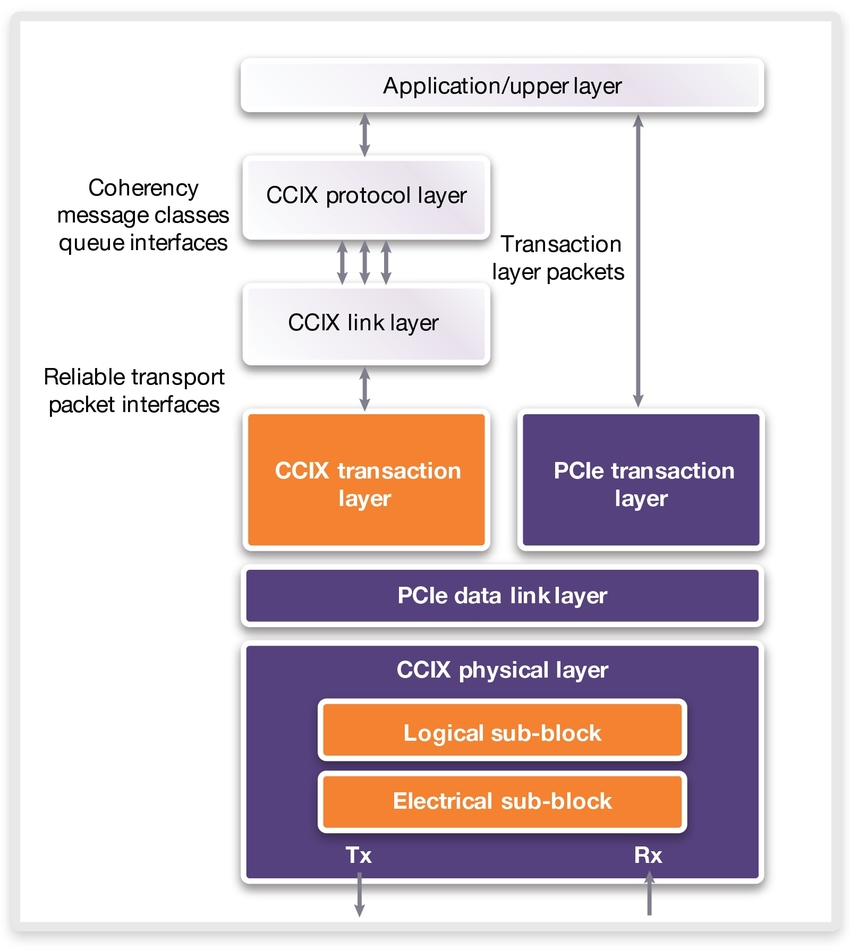
\includegraphics[width=0.50\textwidth]{3-ccix.jpg}
  \caption{Layering diagram of the CCIX standard \cite{using-ccix}.}
  \label{fig:3-ccix}
\end{figure}

The standard supports peer-to-peer and switched topologies with unidirectional bandwidths between \SI{1}{\giga\bit\per\second} and \SI{3.125}{\giga\bit\per\second} per lane. Links consist of eight or sixteen lanes. It provides full cache coherence between the processor and accelerators. Communication with CCIX-attached devices is managed by vendor-specific drivers and libraries.\\
During the typical PCI Express initialization process, the highest mutually supported transfer speed is determined between the two CCIX components. Software running on the host checks configuration registers on the attached device to decide on the transfer speed.





\section{AMBA AXI}
The Advanced Microcontroller Bus Architecture (AMBA) is an open standard by ARM for interconnect protocols. Today, protocols from AMBA are the \textit{de facto} standard in the world of ASICs, FPGAs, SoCs and embedded devices for communication between cores and between cores and attached devices. Currently, FPGAs mostly use the Advanced eXtensible Interface (AXI) protocol by AMBA that will be discussed in this section.



\subsection{Architecture}
While AMBA owns multiple interconnect standards, AXI is the most widely used standard in the world of FPGAs. An example is the abundant use of it in the Xilinx FPGA tool chain and all hardware modules available in the SNAP framework. The latest generation of AXI was released in 2010 in the fourth iteration of the AMBA specification \cite{amba4}.\\
AXI targets high performance and high clock frequency systems by providing a memory-mapped interface that consists of five independent channels: read address, read data, write address, write data, and write response. AXI does not define a specific clock frequency or data width in order to serve the needs for multiple requirements. As an example, the Xilinx AXI generated modules can be configured with a data width of up to 1024 bits \cite{xilinx-pg059}. The frequency depends on the FPGA used in this case and could be in the order of \SI{250}{\mega\hertz} \cite{fuchs}.



\subsection{Handshake Protocol}
The simple uni-directional protocol employs a ready-valid handshake to support flow control in both directions \cite{xilinx-xapp1293}. In essence, the master provides data with an associated valid signal and the slave indicates when it is ready by asserting a ready signal. When at a rising clock edge both valid and ready signals are asserted, data is transferred and both signals are deasserted again.

    

\subsection{AXI Protocol Derivatives}
AXI allows for bursts of data of up to 256 transfer cycles with a single address phase. A derivative is the AXI-Lite standard that is mostly used for low-throughput memory-mapped data transfers. In comparison to AXI, it does not support burst transfers but instead only the transfer of an address-data pair. Another derivative is AXI-Stream, used specifically for streaming applications. The complex address channels are removed and only the ready-valid handshake signals are left. This results in the simplest interface within the AXI family.



\subsection{AXI Coherence Extension}
The AXI Coherence Extension (ACE) \cite{amba4} is an extension to the fourth iteration AMBA specification introduced in 2011. ACE introduces additional signals to enable system-wide coherence \cite{axi-coherence}.\\
The introduction of ACE enabled heterogeneous SoCs such as the ARM big.LITTLE architecture. A derivative of ACE called ACE-Lite enables IO coherency in the sense that an attached device can read from the cache present in the ACE-capable host processor.

%\todo{
%- info on ACE = AXI coherence extension. Problem is that for example hard interconnect IP can be supplied, like CCI-400, with a predefined set of ports. That means little flexibility.\\
%}



%\subsection{CHI}
%\todo{
%- recently announced AMBA5 CHI \url{https://www.arm.com/about/newsroom/arm-announces-amba-5-chi-specification-to-enable-high-performance-highly-scalable-system-on-chip.php} and AHB standards. I downloaded both standards.\\
%}



%\todo{\url{https://community.arm.com/processors/f/discussions/6666/why-is-there-an-acp-interface-for-many-arm-processors}\\
%What is ACP?

%Most of ARM's MPCore processors include an ACP, or Accelerator Coherency Port.  ACPs are just AXI slave ports.  You can connect an AXI master to the port, and the transactions generated by that master will pass through the MPCore processor in order to reach the main memory system.

%Why?

%This is a way of taking a non-cache coherent master and making it cache coherent.

%As the master's transactions pass through the processor, they are visible to the coherency logic in the processor.  This means that should they access an address held in the processor's caches, it can take the necessary steps to ensure coherency. Exactly how this works is down to the specific MPCore processor.

%Note: In practice, it would have to be a non-cached master.  As the ACP only gives visibility of the bus transactions, not any up-stream caches.

%Who initiates transactions over ACP?
%The master (the thing you connected to the ACP). From its perspective not much has changed.

%Check link for more information.
%}




\newpage
\section{Interconnect Comparison}
The preceding sections provided information about the state-of-the-art interconnects. This section summarizes their main characteristics and compares them to the desired requirements for future interconnects discussed in Section \ref{sec:trends-interconnect}.



\subsection{Bandwidth and Latency}
In order to compare various interconnect standards in more detail, the protocols involved and the system that is used should be investigated in more detail. Protocol overhead in transmitted data is for example not taken into account in the comparison presented in \autoref{tab:comparison}, nor are other factors such as packet overhead, and how acknowledge packets incluence bandwidth. System parameters can also affect performance such as payload size and the topology of the interconnect \cite{pcie-xilinx}. With a switched topology, packet congestion can occur if multiple endpoints make multiple requests simultaneously. Determining the latency has similar difficulties in that it depends on so many factors.\\
In general, there is a clear trend to increase the per lane transmission rate in order to provide for example enough bandwidth to accelerators for emerging workloads such as big data and machine learning.



\subsection{Address Space}
There is a trend towards a shared memory model and coherent interconnect with more bandwidth and lower latency. A shared address space across the host and attached devices simplifies the programming model and allows for new use cases.\\
Since PCI Express Gen 3, ATS is included in the specification and enables an ATC on attached devices. While this improves address translations, it does not share a translation table with the host processor as CAPI and OpenCAPI do. Therefore, emerging use cases are not yet possible on PCI Express nor on CCIX.



\subsection{Coherence}
Hardware-based coherence across host cores and attached devices should greatly simplify the programming model.\\
PCI Express uses a snoop filter to keep host caches coherent when host memory is accessed by the attached device. While this improves performance by decreasing data access latency, no coherent cache is present on the attached device itself. CAPI does support a coherent cache on the attached device at the cost of an increased protocol overhead. OpenCAPI will support this in the next generation as well, while currently only coherent memory access is provided. The additional protocol layers of CCIX enable cache coherency and the ACE extension works similarly for AXI interconnects.



\subsection{Synchronization}
With access to shared memory by the attached device, synchronization using shared variables between a thread running on the host and the attached device removes inefficiencies from using interrupts or communication using MMIO registers.\\
PCI Express supports three atomic operations to implement synchronization mechanisms, while CAPI only implements locks. OpenCAPI on the other hand supports multiple atomic operations with a ton of configuration possibilities per operation. This enables a wide variety of synchronization mechanisms to be implemented.

\begin{table}[H]
  \centering
  \caption{Comparison of state-of-the-art interconnect standards.}
  \label{tab:comparison}
  \begin{tabular}{ l | l | l | l | l }
    \textbf{Standard} & \textbf{Bandwidth} & \textbf{Address Space} & \textbf{Coherence} & \textbf{Synchronization} \\ \hline
    PCI Express Gen 3  & \SI{16.0}{\giga\byte\per\second}  & ATS     & Snoop   & Atomics \\
    PCI Express Gen 4  & \SI{32.0}{\giga\byte\per\second}  & ATS     & Snoop   & Atomics \\
    PCI Express Gen 5  & \SI{64.0}{\giga\byte\per\second}  & ATS     & Snoop   & Atomics \\
    CAPI 1.0    & \SI{16.0}{\giga\byte\per\second}  & Shared  & Cache   & Locks   \\
    CAPI 2.0    & \SI{32.0}{\giga\byte\per\second}  & Shared  & Cache   & Unknown \\
    OpenCAPI 3  & \SI{25.0}{\giga\byte\per\second}  & Shared  & Memory  & Atomics \\
    OpenCAPI 4  & \SI{100.0}{\giga\byte\per\second} & Shared  & Cache   & Atomics \\
    CCIX        & \SI{32.0}{\giga\byte\per\second}  & ATS     & Cache   & Unknown \\
    AXI\footnotemark & \SI{16.0}{\giga\byte\per\second} & Memory Mapped & Cache & Unknown \\
  \end{tabular}
\end{table}

\footnotetext{The bandwidth is calculated as the product of a 512 bit wide data bus operating at \SI{250}{\mega\hertz} as used by the SNAP framework \cite{fuchs}. However, higher bandwidths could be obtained by improving either or both parameters.}



\section{Preliminary Concluding Remarks}
\label{sec:3compare}
It is obvious that many advancements in interconnects have been made recently to bridge the gap between host processor cores and attached devices by tighter coupling and extending common concepts for homogeneous multi-core processors to attached devices.\\
Due to the desire of backwards compatibility, PCI Express is limited in terms of innovation and protocol changes. This resulted in a slow release of the Gen 4 specification. At the same time, multiple initiatives started to develop new interconnect standards such as CAPI, OpenCAPI, and CCIX.\\
Due to the support of higher signaling rates than PCI Express, shared memory with address translation and coherent host memory access, OpenCAPI 3.0 is of special interest during the remainder of this thesis. All of these features allow for new usage models and new workloads to be accelerated. In general, upcoming interconnect standards receive a significant increase in bandwidth and this impacts accelerator architectures and design choices.\\
The objective of the remainder of this thesis is to explore how multiple classes of accelerated workloads can be fed with the same or similar reconfigurable buffer architecture to improve designer adoption of OpenCAPI, or other high-bandwidth interconnects. In order to do so, Chapter 4 provides a deeper understanding of OpenCAPI.




%\todo{Interesting news links:\\
%\url{https://www.nextplatform.com/2017/06/30/infiniband-proprietary-networks-still-rule-real-hpc/}\\
%\url{https://www.nextplatform.com/2017/07/14/system-bottleneck-shifts-pci-express/}\\
%\url{https://www.nextplatform.com/2017/07/12/heart-amds-epyc-comeback-infinity-fabric/}\\

%- For comparison of IO on state of the art processor (Power9, etc) and future trends for the IO speeds\\
%\url{https://www.nextplatform.com/2017/07/10/ethernet-getting-back-moores-law-track/}\\
%}
